\documentclass[aspectratio=169]{beamer}
% packages
\usepackage{multicol}
\usepackage[T2A]{fontenc}
\usepackage[utf8]{inputenc}
\usepackage[english,russian]{babel}
\usepackage{booktabs}
\usepackage{biblatex}
\usepackage{graphicx}
\usepackage{href-ul}
\usepackage{cmap}
\usepackage{svg}

\usepackage{lipsum}

% math packages
\usepackage{amsmath,amsfonts,amssymb,amsthm,mathtools}
\usepackage{mathtext}
\usepackage{icomma}
\usepackage{floatflt}

% settings
\setbeamertemplate{navigation symbols}{}
\setbeamertemplate{section in toc}[sections numbered]
\setlength{\columnseprule}{0.2pt}

%%%%%%%%%%%%%%%%%%%%%%%%%%%%%%%%%%
% Metropolis Theme Configuration %
%%%%%%%%%%%%%%%%%%%%%%%%%%%%%%%%%%

\usetheme[
    %%% main theme %%%
    titleformat=regular, 
    %%% inner theme %%%
    sectionpage=progressbar, % + slide
    %sectionpage=none, % disables section page
    %%% outer theme %%%
    numbering=fraction,
    progressbar=frametitle,
    %%% color theme %%%
    block=transparent,
    background=light
]{metropolis}

%%%%%%%%%%%%% Title %%%%%%%%%%%%%%

\setbeamertemplate{title page}{
  \begin{minipage}[b][\paperheight]{\textwidth}
    \centering  % <-- Center here
    \ifx\inserttitlegraphic\@empty\else\usebeamertemplate*{title graphic}\fi
    \vfill%
    \ifx\inserttitle\@empty\else\usebeamertemplate*{title}\fi
    \ifx\insertsubtitle\@empty\else\usebeamertemplate*{subtitle}\fi
    \usebeamertemplate*{title separator}
    \ifx\beamer@shortauthor\@empty\else\usebeamertemplate*{author}\fi
    \ifx\insertdate\@empty\else\usebeamertemplate*{date}\fi
    \ifx\insertinstitute\@empty\else\usebeamertemplate*{institute}\fi
    \vfill
    \vspace*{1mm}
  \end{minipage}
}

\setbeamertemplate{title}{
%  \raggedright%  % <-- Comment here
  \linespread{1.0}%
  \inserttitle%
  \par%
  \vspace*{0.5em}
}
\setbeamertemplate{subtitle}{
%  \raggedright%  % <-- Comment here
  \insertsubtitle%
  \par%
  \vspace*{0.5em}
}

%%%%%%%%%%%%% Blocks %%%%%%%%%%%%%

% map defaulf block to oldblock
\let\oldblock\block
\let\endoldblock\endblock

% change block by adding smallskip
\renewenvironment{block}[1]
{\begin{oldblock}{#1}
    \smallskip
}
{ 
\end{oldblock}
}

\setbeamerfont{bibliography entry title}{size=}
\setbeamerfont{bibliography entry author}{size=}
\setbeamerfont{bibliography entry location}{size=}
\setbeamerfont{bibliography entry note}{size=}

%%%%%%%%%%%%% Colors %%%%%%%%%%%%%

\setbeamercolor{normal text}{fg=black, bg=white}
\setbeamercolor{progress bar}{fg=normal text.fg, bg=normal text.fg!50!black!30} 
\setbeamercolor{frametitle}{fg=normal text.fg, bg=normal text.bg}

% \definecolor{myblue}{RGB}{52,52,178}
% \setbeamercolor{normal text}{fg=black, bg=white}
% \setbeamercolor{progress bar}{fg=normal text.fg, bg=normal text.fg!50!black!30} 
% \setbeamercolor{frametitle}{fg=myblue, bg=normal text.bg}
% \setbeamercolor{palette primary}{bg=myblue}
% \setbeamercolor{block title}{fg=myblue}
% \setbeamercolor{titlelike}{fg=myblue}
% latin bold lower
\newcommand{\ba}{\mathbf{a}} 
\newcommand{\bc}{\mathbf{c}} 
\newcommand{\be}{\mathbf{e}} 
\newcommand{\bh}{\mathbf{h}} 
\newcommand{\bp}{\mathbf{p}} 
\newcommand{\bt}{\mathbf{t}} 
\newcommand{\bs}{\mathbf{s}} 
\newcommand{\bu}{\mathbf{u}} 
\newcommand{\bv}{\mathbf{v}} 
\newcommand{\bw}{\mathbf{w}} 
\newcommand{\bx}{\mathbf{x}} 
\newcommand{\by}{\mathbf{y}} 
\newcommand{\bz}{\mathbf{z}} 
\newcommand{\bm}{\mathbf{m}} 

% latin bold upper
\newcommand{\bA}{\mathbf{A}} 
\newcommand{\bB}{\mathbf{B}} 
\newcommand{\bC}{\mathbf{C}} 
\newcommand{\bI}{\mathbf{I}} 
\newcommand{\bJ}{\mathbf{J}} 
\newcommand{\bL}{\mathbf{L}} 
\newcommand{\bM}{\mathbf{M}} 
\newcommand{\bP}{\mathbf{P}}
\newcommand{\bQ}{\mathbf{Q}} 
\newcommand{\bR}{\mathbf{R}} 
\newcommand{\bT}{\mathbf{T}} 
\newcommand{\bU}{\mathbf{U}} 
\newcommand{\bV}{\mathbf{V}} 
\newcommand{\bW}{\mathbf{W}} 
\newcommand{\bX}{\mathbf{X}} 
\newcommand{\bY}{\mathbf{Y}} 
\newcommand{\bZ}{\mathbf{Z}} 

% latin cal upper
\newcommand{\cF}{\mathcal{F}} 
\newcommand{\cG}{\mathcal{G}} 
\newcommand{\cI}{\mathcal{I}} 
\newcommand{\cL}{\mathcal{L}} 
\newcommand{\cM}{\mathcal{M}} 
\newcommand{\cN}{\mathcal{N}} 
\newcommand{\cS}{\mathcal{S}} 
\newcommand{\cT}{\mathcal{T}} 
\newcommand{\cW}{\mathcal{W}} 
\newcommand{\cX}{\mathcal{X}} 
\newcommand{\cZ}{\mathcal{Z}} 

% latin bb upper
\newcommand{\bbE}{\mathbb{E}} 
\newcommand{\bbI}{\mathbb{I}} 
\newcommand{\bbP}{\mathbb{P}} 
\newcommand{\bbR}{\mathbb{R}}
\newcommand{\bbX}{\mathbb{X}} 
\newcommand{\bbY}{\mathbb{Y}}
\newcommand{\bbW}{\mathbb{W}} 

% greek bold lower
\newcommand{\bepsilon}{\boldsymbol{\epsilon}} 
\newcommand{\btheta}{\boldsymbol{\theta}} 
\newcommand{\blambda}{\boldsymbol{\lambda}} 
\newcommand{\bpi}{\boldsymbol{\pi}} 
\newcommand{\bmu}{\boldsymbol{\mu}} 
\newcommand{\bsigma}{\boldsymbol{\sigma}} 
\newcommand{\bphi}{\boldsymbol{\phi}} 

% greek bold upper
\newcommand{\bSigma}{\boldsymbol{\Sigma}} 

\DeclareMathOperator*{\argmin}{arg\,min}
\DeclareMathOperator*{\argmax}{arg\,max}

% transpose
\newcommand{\T}{^{\text{\tiny\sffamily\upshape\mdseries T}}}
% \addbibresource{references.bib}
\graphicspath{{../paper/figs},{../paper/figs_extraction}}
\usefonttheme[onlymath]{serif}

\newcommand\freefootnote[1]{%
  \let\thefootnote\relax%
  \footnotetext{#1}%
  \let\thefootnote\svthefootnote%
}

%%%
\title{Изменение поверхности функции потерь в нейронных сетях при увеличении размера выборки}
\subtitle{\textcolor{black!50}{Отчет о научно-исследовательской работе}}
\author{
    Киселев Никита Сергеевич\\
    Научный руководитель: к.ф.-м.н. А.\,В.\,Грабовой
}
\date{}
\institute[МФТИ (НИУ)]{
    Московский физико-технический институт\\
    (национальный исследовательский университет)\\
    Физтех-школа прикладной математики и информатики\\
    Кафедра интеллектуальных систем
}
%%%

\begin{document}

\maketitle

\begin{frame}{Изменение поверхности функции потерь}
    Исследуется ландшафт функции потерь в нейронных сетях.
    \begin{block}{Проблема}
        Рассматриваемая поверхность нетривиально зависит от выбранной архитектуры, функции потерь и обучающей выборки. 
    \end{block}
    \begin{block}{Цель}
        Оценить изменение поверхности функции потерь при изменении обучающего набора данных.
    \end{block}
    \begin{block}{Решение}
        \begin{enumerate}
            \item Рассмотреть изменение функции потерь в окрестности минимума при добавлении одного нового объекта;
            \item Использовать аппроксимацию второго порядка в окрестности экстремума.
        \end{enumerate}
    \end{block}
\end{frame}

\begin{frame}{Обзор полученных результатов}
    \begin{figure}[ht]
        \centering
        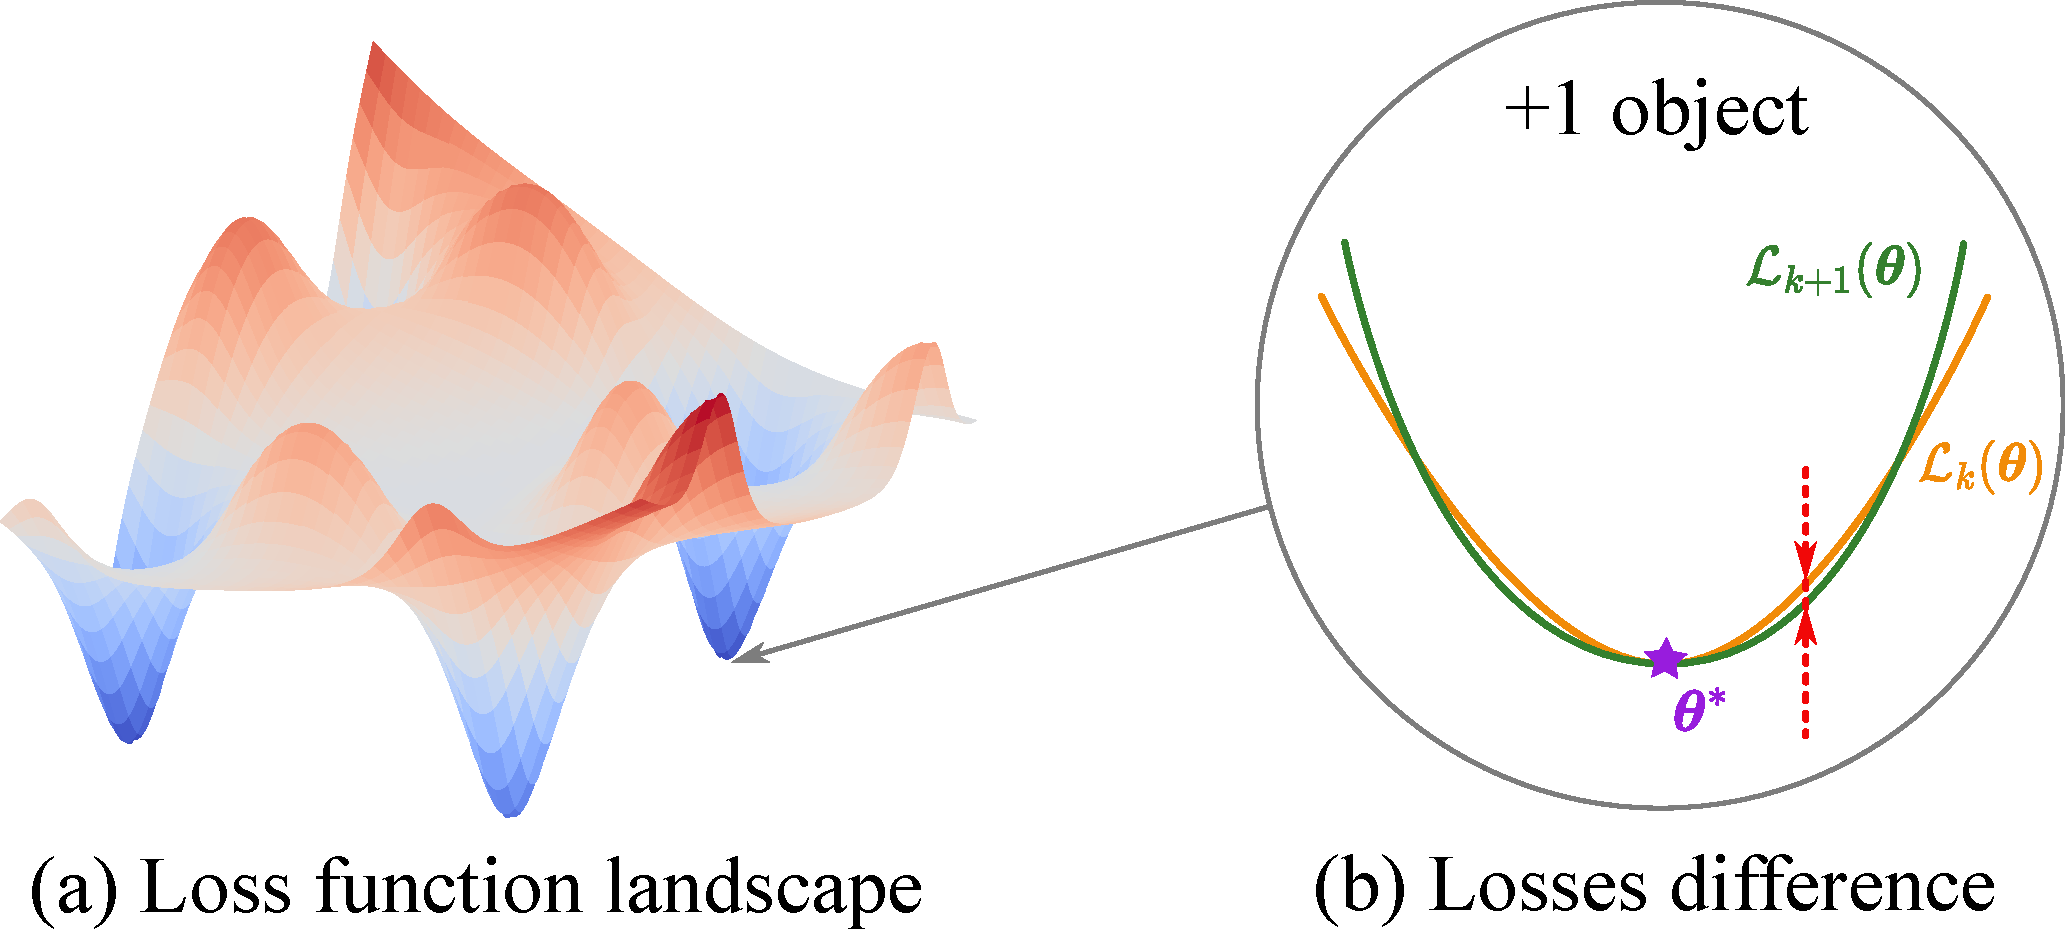
\includegraphics[width=0.65\linewidth]{../paper/losses_difference.pdf}
        \caption{\textbf{Обзор результатов исследования.} Часть (a) показывает ландшафт функции потерь, который является поверхностью в пространстве параметров. Часть (b) показывает разность значений функции ошибки. Она возникает, когда в выборку добавляется один новый объект. Здесь мы демонстрируем поведение для двумерного пространства параметров. Рядом с точкой минимума $\boldsymbol{\theta}^*$ среднее значение функции ошибки на $k+1$ объектах $\mathcal{L}_{k+1}(\boldsymbol{\theta})$ стремится к тому же, но на $k$ объектах $\mathcal{L}_{k}(\boldsymbol{\theta})$.}
    \end{figure}
\end{frame}

\begin{frame}{Обозначения}
    \begin{block}{Выборка}
        \[ \mathfrak{D} = \left\{ (\mathbf{x}_i, \mathbf{y}_i) \right\}, \quad i = 1, \ldots, m, \quad \mathbf{x} \in \mathcal{X}, \ \mathbf{y} \in \mathcal{Y} \]
    \end{block}
    \begin{block}{Модель}
        Условное распределение $p(\mathbf{y}|\mathbf{x})$ аппроксимируется $f_{\boldsymbol{\theta}}: \mathcal{X} \to \mathcal{Y}$, $\boldsymbol{\theta} \in \mathbb{R}^{P}$.
    \end{block}
    \begin{block}{Функция потерь}
        \[ \mathcal{L}_m(\boldsymbol{\theta}) = \dfrac{1}{m} \sum\limits_{i=1}^{m} \ell(f_{\boldsymbol{\theta}}(\mathbf{x}_i), \mathbf{y}_i) \approx \mathbb{E}_{(\mathbf{x}, \mathbf{y}) \sim p(\mathbf{x}, \mathbf{y})} \left[ \ell(f_{\boldsymbol{\theta}}(\mathbf{x}), \mathbf{y}) \right] \]
    \end{block}
    \vspace{-1em}
    \begin{block}{Изменение значения при добавлении одного объекта}
        \begin{equation*}
            \mathcal{L}_{k+1}(\boldsymbol{\theta}) - \mathcal{L}_k(\boldsymbol{\theta}) = \dfrac{1}{k+1} \left( \ell(f_{\boldsymbol{\theta}}(\mathbf{x}_{k+1}), \mathbf{y}_{k+1}) - \mathcal{L}_{k}(\boldsymbol{\theta}) \right)
        \end{equation*}
    \end{block}
\end{frame}

\begin{frame}{Предположение о точке минимума}
    \begin{block}{Предположение 1}
        \vspace{-0.5em}
        Пусть $\boldsymbol{\theta}^*$ является точкой минимума обеих функций $\mathcal{L}_{k}(\boldsymbol{\theta})$ и $\mathcal{L}_{k+1}(\boldsymbol{\theta})$, то есть $\nabla \mathcal{L}_{k}(\boldsymbol{\theta}^*) = \nabla \mathcal{L}_{k+1}(\boldsymbol{\theta}^*) = \mathbf{0}$.
    \end{block}
    \vspace{-0.5em}
    \begin{block}{Аппроксимация второго порядка}
        \vspace{-1em}
        \[ \mathbf{H}^{(k)}(\boldsymbol{\theta}) = \nabla^2_{\boldsymbol{\theta}} \mathcal{L}_{k}(\boldsymbol{\theta}) = \dfrac{1}{k} \sum\limits_{i=1}^{k} \nabla^2_{\boldsymbol{\theta}} \ell(f_{\boldsymbol{\theta}}(\mathbf{x}_{i}), \mathbf{y}_{i}) = \dfrac{1}{k} \sum\limits_{i=1}^{k} \mathbf{H}_{i}(\boldsymbol{\theta}) \]
        \vspace{-0.5em}
        \begin{equation*}
            \mathcal{L}_{k}(\boldsymbol{\theta}) \approx \mathcal{L}_{k}(\boldsymbol{\theta}^*) + \dfrac{1}{2} (\boldsymbol{\theta} - \boldsymbol{\theta}^*)\T \mathbf{H}^{(k)}(\boldsymbol{\theta}^*) (\boldsymbol{\theta} - \boldsymbol{\theta}^*)
        \end{equation*}
    \end{block}
    \vspace{-1em}
    \begin{block}{Абсолютное изменение функции потерь}
        \vspace{-0.7em}
        \[ \left| \mathcal{L}_{k+1}(\boldsymbol{\theta}) - \mathcal{L}_k(\boldsymbol{\theta}) \right| \leqslant \dfrac{1}{k+1} \left| \ell(f_{\boldsymbol{\theta}^*}(\mathbf{x}_{k+1}), \mathbf{y}_{k+1}) - \dfrac{1}{k} \sum\limits_{i=1}^{k} \ell(f_{\boldsymbol{\theta}^*}(\mathbf{x}_{i}), \mathbf{y}_{i}) \right| + \]
        \vspace{-0.5em}
        \[ + \dfrac{1}{k+1} \left\|\boldsymbol{\theta} - \boldsymbol{\theta}^*\right\|_2^2 \left\| \mathbf{H}_{k+1}(\boldsymbol{\theta}^*) - \dfrac{1}{k} \sum\limits_{i=1}^{k} \mathbf{H}_{i}(\boldsymbol{\theta}^*) \right\|_2 \]
    \end{block}
\end{frame}

\begin{frame}{Декомпозиция Гессиана и полносвязная нейронная сеть}
    \begin{block}{Декомпозиция Гессиана}
        \vspace{-0.5em}
        \[
            \mathbf{H}_{i}(\boldsymbol{\theta}) = \underbrace{\nabla_{\boldsymbol{\theta}} \mathbf{z}_i \dfrac{\partial^2 \ell(\mathbf{z}_i, \mathbf{y}_i)}{\partial \mathbf{z}_{i}^2} \nabla_{\boldsymbol{\theta}} \mathbf{z}_i\T }_{\text{G-term}} + \underbrace{\sum\limits_{k=1}^{K} \dfrac{\partial \ell(\mathbf{z}_i, \mathbf{y}_i)}{\partial z_{ik}} \nabla^2_{\boldsymbol{\theta}} z_{ik}}_{\text{H-term}}
        \]
    \end{block}
    \vspace{-2em}
    \begin{block}{Аппроксимация Гессиана}
        В задаче $K$-классовой классификации спектр Гессиана состоит из двух частей\footnote{\scriptsize{Sagun, L. et al. (2017). Empirical analysis of the hessian of over-parametrized neural networks.\\Papyan, V. (2018). The full spectrum of deepnet hessians at scale: Dynamics with sgd training and sample size.\\Ghorbani, B. et al. (2019). An Investigation into Neural Net Optimization via Hessian Eigenvalue Density.}}: ``bulk'' (большое количество около нуля) и ``outliers'' (ровно $K$ ненулевых). Поэтому часто для изучения нормы Гессиана пренебрегают $H$-членом, то есть
        \[ \mathbf{H}_{i}(\boldsymbol{\theta}) \approx \nabla_{\boldsymbol{\theta}} \mathbf{z}_i \dfrac{\partial^2 \ell(\mathbf{z}_i, \mathbf{y}_i)}{\partial \mathbf{z}_{i}^2} \nabla_{\boldsymbol{\theta}} \mathbf{z}_i\T. \]
    \end{block}
\end{frame}

\begin{frame}{Гессиан полносвязной нейронной сети}
    \begin{block}{Полносвязная нейронная сеть}
        Пусть $\mathbf{x} \in \mathbb{R}^{n}$, $\mathbf{y} \in \mathbb{R}^K$. Рассмотрим $L$-слойную сеть для задачи классификации, то есть $f_{\boldsymbol{\theta}}(\mathbf{x}) = \mathbf{z}$ и $\ell(\mathbf{z}, \mathbf{y}) = \mathrm{CE}(\mathbf{p}, \mathbf{y}) = - \sum_{k=1}^{K} y_k \log p_k$:
        \begin{align*}
            &\mathbf{z}^{(p)} = \mathbf{W}^{(p)} \mathbf{x}^{(p)} + \mathbf{b}^{(p)}, \\
            &\mathbf{x}^{(p+1)} = \sigma(\mathbf{z}^{(p)}),
        \end{align*}
        где $\mathrm{softmax}{(\mathbf{z})} = \mathbf{p}$, а $\sigma(\mathbf{x}) = \left[ \mathbf{x} \geqslant \mathbf{0} \right] \mathbf{x}$ есть функция активации ReLU. 

        
    \end{block}
\end{frame}

\begin{frame}{Аппроксимация Гессиана полносвязной сети на одном объекте}
    \vspace{-0.5em}
    \[ \fbox{$\mathbf{H}(\boldsymbol{\theta}) \stackrel{2}{\approx} \mathbf{F}\T \mathbf{A} \mathbf{F}$} \]
    \vspace{-2em}
    \begin{itemize}
        \item $\mathbf{D}^{(p)} = \mathrm{diag}([\mathbf{z}^{(p)} \geqslant \mathbf{0}])$
        \item $\mathbf{G}^{(p)} = \dfrac{\partial \mathbf{z}}{\partial \mathbf{z}^{(p)}} = \mathbf{W}^{(L)} \mathbf{D}^{(L-1)} \mathbf{W}^{(L-1)} \mathbf{D}^{(L-2)} \cdot \ldots \cdot \mathbf{D}^{(p)}$
        \item 
        \[ \mathbf{F}\T = \begin{pmatrix}
            (\mathbf{G}^{(1)})\T \otimes \mathbf{x}^{(1)} \\
            (\mathbf{G}^{(1)})\T \\ 
            \vdots \\
            (\mathbf{G}^{(L)})\T \otimes \mathbf{x}^{(L)} \\
            (\mathbf{G}^{(L)})\T \\ 
        \end{pmatrix} \]
        \item $\mathbf{A} = \nabla^2_\mathbf{z} \ell(\mathbf{z}, \mathbf{y}) = \mathrm{diag}(\mathbf{p}) - \mathbf{p} \mathbf{p}\T$
    \end{itemize}
    \vspace{1em}
    \freefootnote{$^2$Wu, Y. et al. (2020). Dissecting hessian: Understanding common structure of hessian in neural networks.}
\end{frame}

\begin{frame}{Ограниченность и пропорциональность нормы Гессиана}
    \fontsize{9pt}{10pt}\selectfont
    \vspace{1em}
    \begin{block}{Теорема 1 (об ограниченности нормы Гессиана)}
        \vspace{-0.5em}
        Пусть задана $L$-слойная полносвязная нейронная сеть с функцией активацией ReLU и без параметров смещения, применямая для решения задачи $K$-классовой классификации. Если выполнено следующее: $\| \mathbf{W}^{(p)} \|_2 \leqslant M_{\mathbf{W}}$ и $\| \mathbf{x}_i \|_2 \leqslant M_{\mathbf{x}}$ для всех слоев $p = 1, \ldots, L$ в сети и для всех объектов $i = 1, \ldots, m$ в наборе данных, то для любого объекта $i = 1, \ldots, m$ верно следующее неравенство:
        \vspace{-1em}
        \[ \left\| \mathbf{H}_i(\boldsymbol{\theta}) \right\|_2 \leqslant L \sqrt{2} M_{\mathbf{x}}^2 M_{\mathbf{W}}^{2L} + \sqrt{2} \dfrac{M_{\mathbf{W}}^2 (M_{\mathbf{W}}^{2L} - 1)}{M_{\mathbf{W}}^2 - 1}. \]
    \end{block}
    \vspace{-1.25em}
    \begin{block}{Лемма 1 (о пропорциональности нормы Гессиана)}
        \vspace{-0.5em}
        Если каждый параметр модели ограничен константой $M > 0$, то есть $|w_{ij}^{(p)}| \leqslant M$ для всех $i, j = 1, \ldots, h$ и для всех слоев $p = 1, \ldots, L$, тогда в условиях Теоремы~1 верно следующее:
        \vspace{-0.5em}
        \[ \left\| \mathbf{H}_i(\boldsymbol{\theta}) \right\|_2 \leqslant L \sqrt{2} M_{\mathbf{x}}^2 (hM)^{2L} + \sqrt{2} \dfrac{(hM)^2 ((hM)^{2L} - 1)}{(hM)^2 - 1}. \]
        \vspace{-0.5em}
        Таким образом, верна следующая пропорция:
        \vspace{-0.5em}
        \[ \left\| \mathbf{H}_i(\boldsymbol{\theta}) \right\|_2 \propto L (hM)^{2L}. \]
    \end{block}
\end{frame}

\begin{frame}{Сходимость абсолютной разности функции потерь}
    \fontsize{9pt}{10pt}\selectfont
    \vspace{1em}
    \begin{block}{Лемма 2 (о сходимости абсолютной разности функции потерь)}
        Пусть точка $\boldsymbol{\theta}$ выбрана так, что $\left\|\boldsymbol{\theta} - \boldsymbol{\theta}^*\right\|_2^2 \leqslant R^2$ для некоторого $R > 0$. Если существует неотрицательная константа $M_{\ell}$, что $\left| \ell(f_{\boldsymbol{\theta}^*}(\mathbf{x}_{i}), \mathbf{y}_{i}) \right| \leqslant M_{\ell}$ для всех объектов $i = 1, \ldots, m$ в наборе данных, то в условиях Теоремы~1 верно следующее:
        \[ \left| \mathcal{L}_{k+1}(\boldsymbol{\theta}) - \mathcal{L}_k(\boldsymbol{\theta}) \right| \leqslant \dfrac{2}{k+1}\left( M_{\ell} + \left( L \sqrt{2} M_{\mathbf{x}}^2 M_{\mathbf{W}}^{2L} + \sqrt{2} \dfrac{M_{\mathbf{W}}^2 (M_{\mathbf{W}}^{2L} - 1)}{M_{\mathbf{W}}^2 - 1} \right) R^2 \right) \to 0 \text{ при } k \to \infty. \]
        Таким образом, верна следующая пропорция:
        \begin{equation*}
            \left| \mathcal{L}_{k+1}(\boldsymbol{\theta}) - \mathcal{L}_k(\boldsymbol{\theta}) \right| \propto \dfrac{L (hM)^{2L} R^2}{k}. 
        \end{equation*}
    \end{block}
\end{frame}

\section{Вычислительный эксперимент}

\begin{frame}{Постановка эксперимента}
    \begin{itemize}
        \item \textbf{Задача:} классификация изображений:
        \begin{enumerate}
            \item Прямая, то есть пиксели есть признаки,
            \item С предварительной векторизацией при помощи предобученной модели ViT;
        \end{enumerate}
        \item \textbf{Выборка:} MNIST, FashionMNIST, CIFAR10, CIFAR100;
        \item \textbf{Архитектура:} полносвязная $L$-слойная сеть со скрытым размером $h$ на каждом слое и ReLU после каждого из них;
        \item \textbf{Варьирование архитектуры:}
        \begin{enumerate}
            \item Фиксируем число слоев $L$ и варьируем размер скрытого слоя $h$,
            \item Наоборот, фиксируем размер скрытого слоя $h$ и варьируем число слоев $L$;
        \end{enumerate}
        \item \textbf{Постановка эксперимента:}
        \begin{enumerate}
            \item Обучаем модель на полном наборе данных $\to$ получаем $\hat{\boldsymbol{\theta}}$,
            \item Подсчитываем $\left| \mathcal{L}_{k+1}(\hat{\boldsymbol{\theta}}) - \mathcal{L}_k(\hat{\boldsymbol{\theta}}) \right|$ для всех $k = 1, \ldots, m$,
            \item Повторяем пункт 2 несколько раз, используя разный порядок добавления.
        \end{enumerate}
    \end{itemize}
\end{frame}

\begin{frame}{Прямая классификация изображений}
    \begin{figure}[ht]
        \centering
        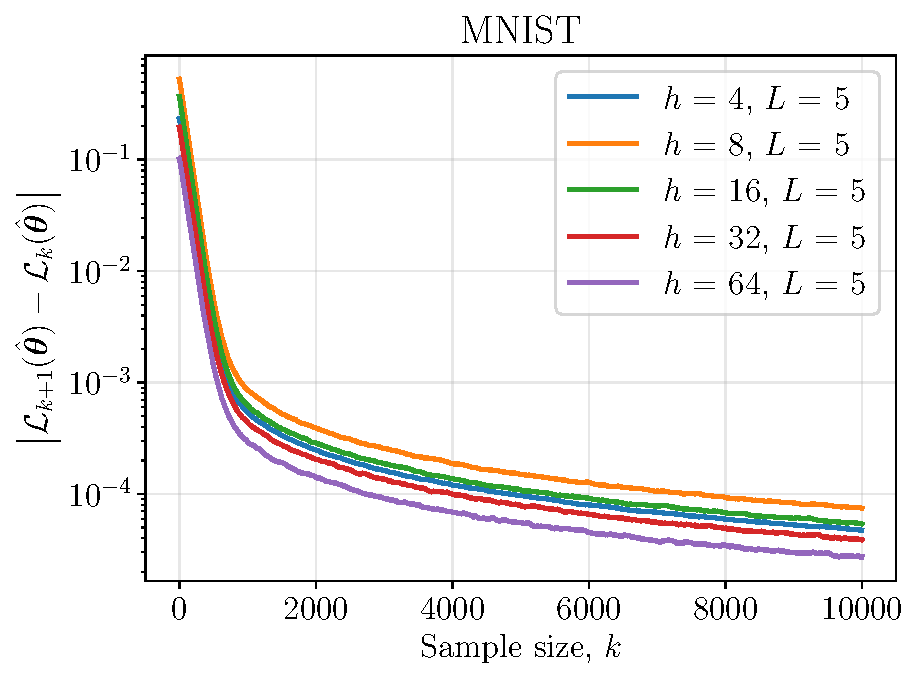
\includegraphics[width=0.5\linewidth]{../paper/figs/mnist_hidden_size.pdf}\hfill
        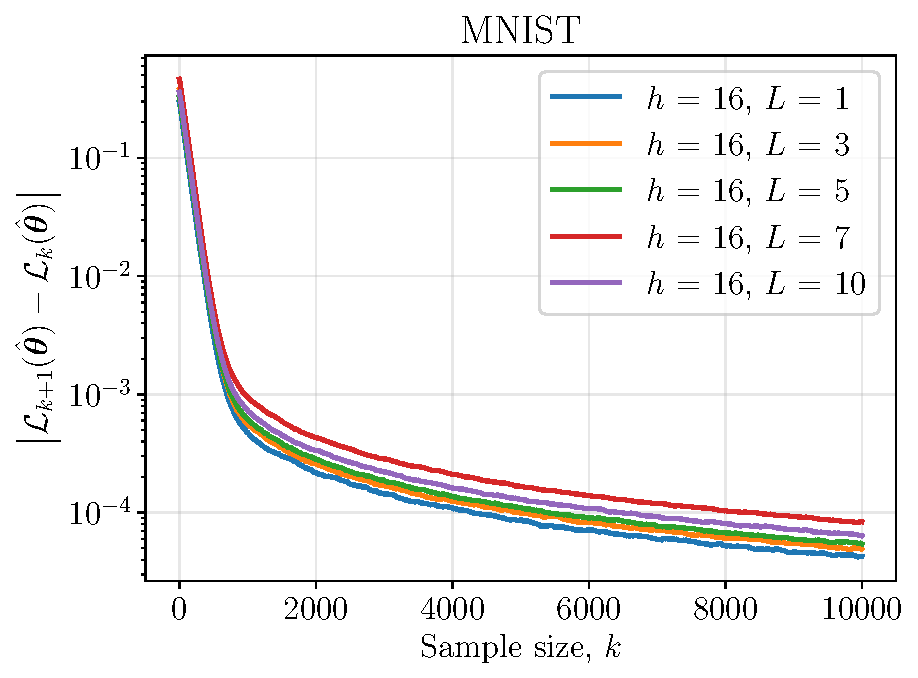
\includegraphics[width=0.5\linewidth]{../paper/figs/mnist_num_layers.pdf}
        \caption{Зависимость абсолютного значения разности значений функции ошибки от доступного размера выборки, на задаче прямой классификации изображений. Графики слева демонстрируют уменьшение значений при увеличении размера скрытого слоя. Графики справа демонстрируют увеличение значений при увеличении числа слоев.}
    \end{figure}
\end{frame}

\begin{frame}{Предварительная векторизация изображений}
    \begin{figure}[ht]
        \centering
        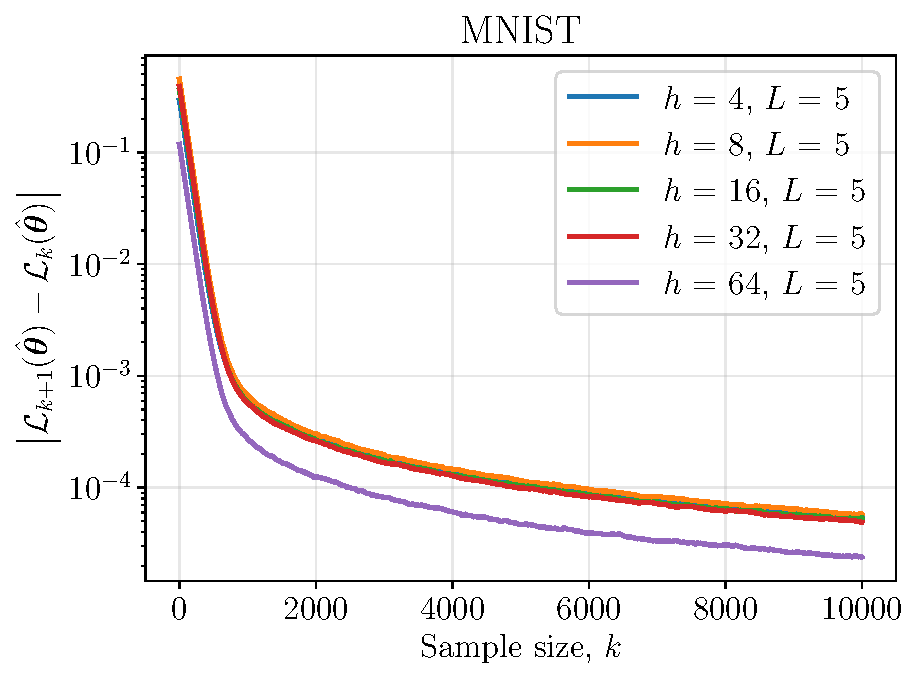
\includegraphics[width=0.5\linewidth]{../paper/figs_extraction/mnist_hidden_size.pdf}\hfill
        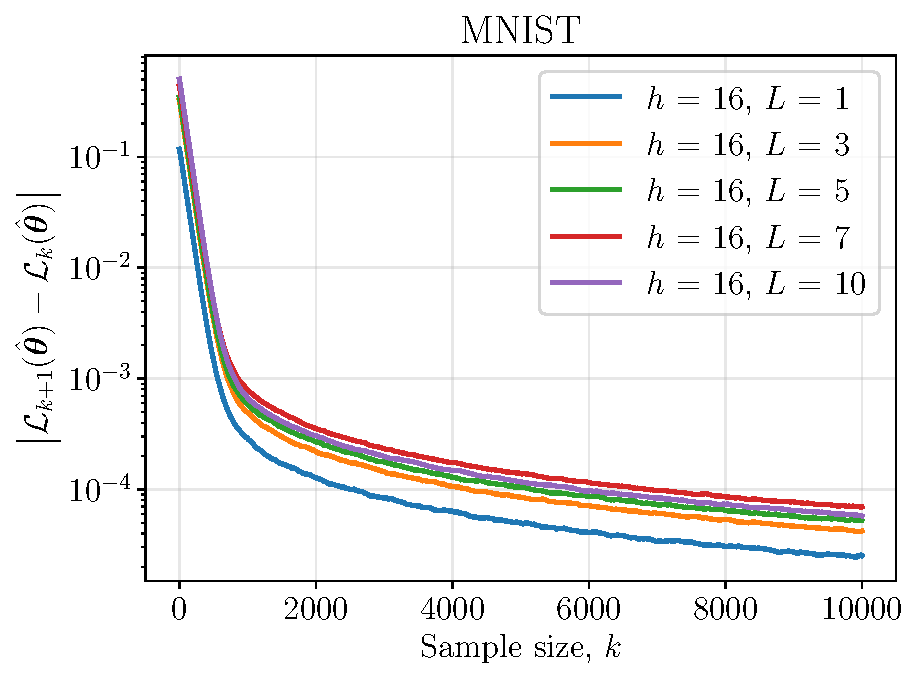
\includegraphics[width=0.5\linewidth]{../paper/figs_extraction/mnist_num_layers.pdf}
        \caption{Зависимость абсолютного значения разности значений функции ошибки от доступного размера выборки, на задаче с предварительной векторизацией изображений. Графики слева демонстрируют уменьшение значений при увеличении размера скрытого слоя. Графики справа демонстрируют увеличение значений при увеличении числа слоев.}
    \end{figure}
\end{frame}

\begin{frame}{Заключение}
    \begin{enumerate}
        \item Доказаны теоретические результаты о сходимости поверхности функции потерь в полносвязной нейронной сети при увеличении размера выборки;
        \item Вычислительный эксперимент демонстрирует справедливость полученных результатов на практике;
        \item Дальнейшее исследование лежит в направлении 1) рассмотрения других архитектур\footnote{Ожидается выступление студента 4-го курса Владислава Мешкова на конференции ИСП РАН по совместному исследованию для сверточных архитектур}, 2) определения достаточного размера выборки.
    \end{enumerate}
    \begin{block}{Публикации}
        \begin{enumerate}
            \item N.~Kiselev, A.~Grabovoy. Unraveling the Hessian: A Key to Smooth Convergence in Loss Function Landscapes // arXiv preprint arXiv:2409.11995. – 2024.\\
            Отобрана для публикации в рамках конференции AI Journey 2024. Будет опубликована в журнале Doklady Mathematics (\textbf{Q2}).
        \end{enumerate}
    \end{block}
    \vspace{0.5em}
\end{frame}

\end{document}